

\documentclass{article}

\usepackage{pgfplots}
\pgfplotsset{compat = newest}
\usepackage{titlesec}
\usepackage{graphicx}
\usepackage{wrapfig}
\usepackage{amsfonts}
\usepackage{tikz}
\usepackage{amssymb}
\usepackage{amsfonts}
\usepackage{amsmath}

\begin{document}

\section*{Homework Questions}

(about the lottery scheduler)

\begin{enumerate}

    \item \textbf{Compute the solutions for simulations with 3 jobs and random seeds of 1, 2, and 3.}\\\\
    \underline{seed 1}
    \begin{verbatim}
    python lottery.py -j 3 -s 1 -c
    ARG jlist 
    ARG jobs 3
    ARG maxlen 10
    ARG maxticket 100
    ARG quantum 1
    ARG seed 1
    
    Here is the job list, with the run time of each job: 
        Job 0 ( length = 1, tickets = 84 )
        Job 1 ( length = 7, tickets = 25 )
        Job 2 ( length = 4, tickets = 44 )
    
    ** Solutions **
    
    Random 651593 -> Winning ticket 119 (of 153) -> Run 2
        Jobs:
        (  job:0 timeleft:1 tix:84 )  (  job:1 timeleft:7 tix:25 )  (* job:2 timeleft:4 tix:44 ) 
    Random 788724 -> Winning ticket 9 (of 153) -> Run 0
        Jobs:
        (* job:0 timeleft:1 tix:84 )  (  job:1 timeleft:7 tix:25 )  (  job:2 timeleft:3 tix:44 ) 
    --> JOB 0 DONE at time 2
    Random 93859 -> Winning ticket 19 (of 69) -> Run 1
        Jobs:
        (  job:0 timeleft:0 tix:--- )  (* job:1 timeleft:7 tix:25 )  (  job:2 timeleft:3 tix:44 ) 
    Random 28347 -> Winning ticket 57 (of 69) -> Run 2
        Jobs:
        (  job:0 timeleft:0 tix:--- )  (  job:1 timeleft:6 tix:25 )  (* job:2 timeleft:3 tix:44 ) 
    Random 835765 -> Winning ticket 37 (of 69) -> Run 2
        Jobs:
        (  job:0 timeleft:0 tix:--- )  (  job:1 timeleft:6 tix:25 )  (* job:2 timeleft:2 tix:44 ) 
    Random 432767 -> Winning ticket 68 (of 69) -> Run 2
        Jobs:
        (  job:0 timeleft:0 tix:--- )  (  job:1 timeleft:6 tix:25 )  (* job:2 timeleft:1 tix:44 ) 
    --> JOB 2 DONE at time 6
    Random 762280 -> Winning ticket 5 (of 25) -> Run 1
        Jobs:
        (  job:0 timeleft:0 tix:--- )  (* job:1 timeleft:6 tix:25 )  (  job:2 timeleft:0 tix:--- ) 
    Random 2106 -> Winning ticket 6 (of 25) -> Run 1
        Jobs:
        (  job:0 timeleft:0 tix:--- )  (* job:1 timeleft:5 tix:25 )  (  job:2 timeleft:0 tix:--- ) 
    Random 445387 -> Winning ticket 12 (of 25) -> Run 1
        Jobs:
        (  job:0 timeleft:0 tix:--- )  (* job:1 timeleft:4 tix:25 )  (  job:2 timeleft:0 tix:--- ) 
    Random 721540 -> Winning ticket 15 (of 25) -> Run 1
        Jobs:
        (  job:0 timeleft:0 tix:--- )  (* job:1 timeleft:3 tix:25 )  (  job:2 timeleft:0 tix:--- ) 
    Random 228762 -> Winning ticket 12 (of 25) -> Run 1
        Jobs:
        (  job:0 timeleft:0 tix:--- )  (* job:1 timeleft:2 tix:25 )  (  job:2 timeleft:0 tix:--- ) 
    Random 945271 -> Winning ticket 21 (of 25) -> Run 1
        Jobs:
        (  job:0 timeleft:0 tix:--- )  (* job:1 timeleft:1 tix:25 )  (  job:2 timeleft:0 tix:--- ) 
    --> JOB 1 DONE at time 12
    \end{verbatim}
    \underline{seed 2}
    \begin{verbatim}
    python lottery.py -j 3 -s 2 -c
    ARG jlist 
    ARG jobs 3
    ARG maxlen 10
    ARG maxticket 100
    ARG quantum 1
    ARG seed 2
    
    Here is the job list, with the run time of each job: 
        Job 0 ( length = 9, tickets = 94 )
        Job 1 ( length = 8, tickets = 73 )
        Job 2 ( length = 6, tickets = 30 )
    
    
    ** Solutions **
    
    Random 605944 -> Winning ticket 169 (of 197) -> Run 2
        Jobs:
        (  job:0 timeleft:9 tix:94 )  (  job:1 timeleft:8 tix:73 )  (* job:2 timeleft:6 tix:30 ) 
    Random 606802 -> Winning ticket 42 (of 197) -> Run 0
        Jobs:
        (* job:0 timeleft:9 tix:94 )  (  job:1 timeleft:8 tix:73 )  (  job:2 timeleft:5 tix:30 ) 
    Random 581204 -> Winning ticket 54 (of 197) -> Run 0
        Jobs:
        (* job:0 timeleft:8 tix:94 )  (  job:1 timeleft:8 tix:73 )  (  job:2 timeleft:5 tix:30 ) 
    Random 158383 -> Winning ticket 192 (of 197) -> Run 2
        Jobs:
        (  job:0 timeleft:7 tix:94 )  (  job:1 timeleft:8 tix:73 )  (* job:2 timeleft:5 tix:30 ) 
    Random 430670 -> Winning ticket 28 (of 197) -> Run 0
        Jobs:
        (* job:0 timeleft:7 tix:94 )  (  job:1 timeleft:8 tix:73 )  (  job:2 timeleft:4 tix:30 ) 
    Random 393532 -> Winning ticket 123 (of 197) -> Run 1
        Jobs:
        (  job:0 timeleft:6 tix:94 )  (* job:1 timeleft:8 tix:73 )  (  job:2 timeleft:4 tix:30 ) 
    Random 723012 -> Winning ticket 22 (of 197) -> Run 0
        Jobs:
        (* job:0 timeleft:6 tix:94 )  (  job:1 timeleft:7 tix:73 )  (  job:2 timeleft:4 tix:30 ) 
    Random 994820 -> Winning ticket 167 (of 197) -> Run 2
        Jobs:
        (  job:0 timeleft:5 tix:94 )  (  job:1 timeleft:7 tix:73 )  (* job:2 timeleft:4 tix:30 ) 
    Random 949396 -> Winning ticket 53 (of 197) -> Run 0
        Jobs:
        (* job:0 timeleft:5 tix:94 )  (  job:1 timeleft:7 tix:73 )  (  job:2 timeleft:3 tix:30 ) 
    Random 544177 -> Winning ticket 63 (of 197) -> Run 0
        Jobs:
        (* job:0 timeleft:4 tix:94 )  (  job:1 timeleft:7 tix:73 )  (  job:2 timeleft:3 tix:30 ) 
    Random 444854 -> Winning ticket 28 (of 197) -> Run 0
        Jobs:
        (* job:0 timeleft:3 tix:94 )  (  job:1 timeleft:7 tix:73 )  (  job:2 timeleft:3 tix:30 ) 
    Random 268241 -> Winning ticket 124 (of 197) -> Run 1
        Jobs:
        (  job:0 timeleft:2 tix:94 )  (* job:1 timeleft:7 tix:73 )  (  job:2 timeleft:3 tix:30 ) 
    Random 35924 -> Winning ticket 70 (of 197) -> Run 0
        Jobs:
        (* job:0 timeleft:2 tix:94 )  (  job:1 timeleft:6 tix:73 )  (  job:2 timeleft:3 tix:30 ) 
    Random 27444 -> Winning ticket 61 (of 197) -> Run 0
        Jobs:
        (* job:0 timeleft:1 tix:94 )  (  job:1 timeleft:6 tix:73 )  (  job:2 timeleft:3 tix:30 ) 
    --> JOB 0 DONE at time 14
    Random 464894 -> Winning ticket 55 (of 103) -> Run 1
        Jobs:
        (  job:0 timeleft:0 tix:--- )  (* job:1 timeleft:6 tix:73 )  (  job:2 timeleft:3 tix:30 ) 
    Random 318465 -> Winning ticket 92 (of 103) -> Run 2
        Jobs:
        (  job:0 timeleft:0 tix:--- )  (  job:1 timeleft:5 tix:73 )  (* job:2 timeleft:3 tix:30 ) 
    Random 380015 -> Winning ticket 48 (of 103) -> Run 1
        Jobs:
        (  job:0 timeleft:0 tix:--- )  (* job:1 timeleft:5 tix:73 )  (  job:2 timeleft:2 tix:30 ) 
    Random 891790 -> Winning ticket 16 (of 103) -> Run 1
        Jobs:
        (  job:0 timeleft:0 tix:--- )  (* job:1 timeleft:4 tix:73 )  (  job:2 timeleft:2 tix:30 ) 
    Random 525753 -> Winning ticket 41 (of 103) -> Run 1
        Jobs:
        (  job:0 timeleft:0 tix:--- )  (* job:1 timeleft:3 tix:73 )  (  job:2 timeleft:2 tix:30 ) 
    Random 560510 -> Winning ticket 87 (of 103) -> Run 2
        Jobs:
        (  job:0 timeleft:0 tix:--- )  (  job:1 timeleft:2 tix:73 )  (* job:2 timeleft:2 tix:30 ) 
    Random 236123 -> Winning ticket 47 (of 103) -> Run 1
        Jobs:
        (  job:0 timeleft:0 tix:--- )  (* job:1 timeleft:2 tix:73 )  (  job:2 timeleft:1 tix:30 ) 
    Random 23858 -> Winning ticket 65 (of 103) -> Run 1
        Jobs:
        (  job:0 timeleft:0 tix:--- )  (* job:1 timeleft:1 tix:73 )  (  job:2 timeleft:1 tix:30 ) 
    --> JOB 1 DONE at time 22
    Random 325143 -> Winning ticket 3 (of 30) -> Run 2
        Jobs:
        (  job:0 timeleft:0 tix:--- )  (  job:1 timeleft:0 tix:--- )  (* job:2 timeleft:1 tix:30 ) 
    --> JOB 2 DONE at time 23
    \end{verbatim}
    \underline{seed 3}
    \begin{verbatim}
    python lottery.py -j 3 -s 3 -c
    ARG jlist 
    ARG jobs 3
    ARG maxlen 10
    ARG maxticket 100
    ARG quantum 1
    ARG seed 3
    
    Here is the job list, with the run time of each job: 
        Job 0 ( length = 2, tickets = 54 )
        Job 1 ( length = 3, tickets = 60 )
        Job 2 ( length = 6, tickets = 6 )
    
    
    ** Solutions **
    
    Random 13168 -> Winning ticket 88 (of 120) -> Run 1
        Jobs:
        (  job:0 timeleft:2 tix:54 )  (* job:1 timeleft:3 tix:60 )  (  job:2 timeleft:6 tix:6 ) 
    Random 837469 -> Winning ticket 109 (of 120) -> Run 1
        Jobs:
        (  job:0 timeleft:2 tix:54 )  (* job:1 timeleft:2 tix:60 )  (  job:2 timeleft:6 tix:6 ) 
    Random 259354 -> Winning ticket 34 (of 120) -> Run 0
        Jobs:
        (* job:0 timeleft:2 tix:54 )  (  job:1 timeleft:1 tix:60 )  (  job:2 timeleft:6 tix:6 ) 
    Random 234331 -> Winning ticket 91 (of 120) -> Run 1
        Jobs:
        (  job:0 timeleft:1 tix:54 )  (* job:1 timeleft:1 tix:60 )  (  job:2 timeleft:6 tix:6 ) 
    --> JOB 1 DONE at time 4
    Random 995645 -> Winning ticket 5 (of 60) -> Run 0
        Jobs:
        (* job:0 timeleft:1 tix:54 )  (  job:1 timeleft:0 tix:--- )  (  job:2 timeleft:6 tix:6 ) 
    --> JOB 0 DONE at time 5
    Random 470263 -> Winning ticket 1 (of 6) -> Run 2
        Jobs:
        (  job:0 timeleft:0 tix:--- )  (  job:1 timeleft:0 tix:--- )  (* job:2 timeleft:6 tix:6 ) 
    Random 836462 -> Winning ticket 2 (of 6) -> Run 2
        Jobs:
        (  job:0 timeleft:0 tix:--- )  (  job:1 timeleft:0 tix:--- )  (* job:2 timeleft:5 tix:6 ) 
    Random 476353 -> Winning ticket 1 (of 6) -> Run 2
        Jobs:
        (  job:0 timeleft:0 tix:--- )  (  job:1 timeleft:0 tix:--- )  (* job:2 timeleft:4 tix:6 ) 
    Random 639068 -> Winning ticket 2 (of 6) -> Run 2
        Jobs:
        (  job:0 timeleft:0 tix:--- )  (  job:1 timeleft:0 tix:--- )  (* job:2 timeleft:3 tix:6 ) 
    Random 150616 -> Winning ticket 4 (of 6) -> Run 2
        Jobs:
        (  job:0 timeleft:0 tix:--- )  (  job:1 timeleft:0 tix:--- )  (* job:2 timeleft:2 tix:6 ) 
    Random 634861 -> Winning ticket 1 (of 6) -> Run 2
        Jobs:
        (  job:0 timeleft:0 tix:--- )  (  job:1 timeleft:0 tix:--- )  (* job:2 timeleft:1 tix:6 ) 
    --> JOB 2 DONE at time 11
    \end{verbatim}

    \item \textbf{Now run with two specific jobs: each of length 10, but one (job 0) with just 1 ticket and the other (job 1) with 100 (e.g., -l 10:1,10:100). What happens when the number of tickets is so imbalanced? Will job 0 ever run before job 1 completes? How often? In general, what does such a ticket imbalance do to the behavior of lottery scheduling?}\\\\
    It is extremely unlikely that job 0 will ever run before job 1 because of the imbalance of tickets. The behaviour changes into more of FIFO scheduling and becomes unfair.

    \item \textbf{When running with two jobs of length 100 and equal ticket alocations of 100 (-l 100:100,100:100), how unfair is the scheduler? Run with some different random seeds to determine the (probalistic) answer; let unfairness be determined by how much earlier one job finishes than the other.} \\\\
    
    Unfairness metric = U \\
    U = the time the first job completes divided by the time the second job completes\\
    (A perfectly fair scheduler achieves U = 1)\\

    (rounded to 2 decimal places)\\\\
    \underline{Run 0}\\
    $s = 0$ \\
    $U = \frac{192}{200} = 0.96$\\\\
    \underline{Run 1}\\
    $s = 1$\\
    $U = \frac{196}{200} = 0.98$\\\\
    \underline{Run 2}\\
    $s = 2$\\
    $U = \frac{190}{200} = 0.95$\\\\
    \underline{Run 3} \\
    $s = 3$\\
    $U = \frac{196}{200} = 0.98$\\\\
    \underline{Run 4}\\
    $s = 4$\\
    $U = \frac{199}{200} = 1.00$\\\\

    So, overall the scheduler is pretty fair.

    \item \textbf{How does your answer to the previous question change as the quantum size (-q) gets larger?}\\\\
    
    - length of time slice in prev question was 1\\\\

    \underline{\textbf{q = 10}}
    \underline{Run 0}\\
    $s = 0$ \\
    $U = \frac{150}{200} = 0.75$\\\\
    \underline{Run 1}\\
    $s = 1$\\
    $U = \frac{160}{200} = 0.80$\\\\
    \underline{Run 2}\\
    $s = 2$\\
    $U = \frac{190}{200} = 0.95$\\\\
    \underline{Run 3} \\
    $s = 3$\\
    $U = \frac{190}{200} = 0.95$\\\\
    \underline{Run 4}\\
    $s = 4$\\
    $U = \frac{190}{200} = 0.95$\\\\

    \underline{\textbf{q = 50}}
    \underline{Run 0}\\
    $s = 0$ \\
    $U = \frac{150}{200} = 0.75$\\\\
    \underline{Run 1}\\
    $s = 1$\\
    $U = \frac{150}{200} = 0.75$\\\\
    \underline{Run 2}\\
    $s = 2$\\
    $U = \frac{100}{200} = 0.50$\\\\
    \underline{Run 3} \\
    $s = 3$\\
    $U = \frac{150}{200} = 0.75$\\\\
    \underline{Run 4}\\
    $s = 4$\\
    $U = \frac{150}{200} = 0.75$\\\\

    As the quantum size gets larger, the scheduler becomes more unfair.

    \item \textbf{Can you make a version of the graph that is found in the chapter? What else would be worth exploring? How would the graph look with a stride scheduler?}
    
    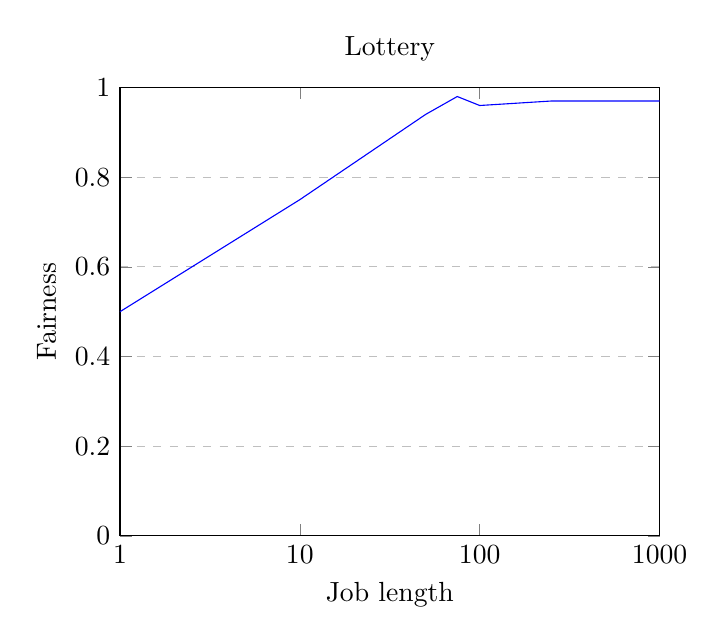
\begin{tikzpicture}
    \begin{axis}[title=Lottery, xlabel={Job length}, ylabel={Fairness},xmin=1,xmax=1000, ymin=0, ymax=1, xtick={1,10,100,1000}, xticklabels={1,10,100,1000}, ytick={0,0.2,0.4,0.6,0.8,1.0}, legend pos=north west, ymajorgrids=true, grid style=dashed, x coord trafo/.code={\pgfmathparse{ln(#1)}\pgfmathresult}, x coord inv trafo/.code={\pgfmathparse{exp(#1)}\pgfmathresult}]

    \addplot[color=blue,]
        coordinates {
        (1,0.5)(10,0.75)(50,0.94)(75,0.98)(100,0.96)(250,0.97)(500,0.97)(750,0.97)(1000,0.97)
        };
    \end{axis}
    \end{tikzpicture}\\

    \begin{tikzpicture}
    \begin{axis}[title =Stride, xlabel={Job length}, ylabel={Fairness},xmin=1,xmax=1000, ymin=0, ymax=1.2, xtick={1,10,100,1000}, xticklabels={1,10,100,1000}, ytick={0,0.2,0.4,0.6,0.8,1.0}, legend pos=north west, ymajorgrids=true, grid style=dashed, x coord trafo/.code={\pgfmathparse{ln(#1)}\pgfmathresult}, x coord inv trafo/.code={\pgfmathparse{exp(#1)}\pgfmathresult}]

    \addplot[color=blue,]
        coordinates {
        (1,1)(10,1)(100,1)(1000,1)
        };
    \end{axis}
    \end{tikzpicture}

\end{enumerate}


\end{document}